% DK: My book is out of print now, but the chapter in Rhythm is available online, http://www.informit.com/articles/article.aspx?p=28785 You might find some ideas that lineup with this pattern there
\section{Heartbeat}\label{sec:Heartbeat}

\subsubsection*{Motivation} This pattern can help project participants stay in touch, and stay motivated.

\subsubsection*{Context}
% DK: I think you might be missing some pieces of context….people are busy, the FLOSS project is probably not their day job, etc…
A number of people have a shared interest, and have connected with each other about it.  However, they are not going to spend 24 hours a day, 7 days a week working together, either because they are busy with other things, or because working separately on some tasks is vastly more efficient.

\subsubsection*{Forces}~
\begin{tabular}[t]{p{.8\textwidth}@{\hspace{.03\textwidth}}c}
\textbf{Differentiation}: the time we spend together isn't all equally meaningful. & {\icon \symbol{"002185}} \\
\textbf{Entropy}: something needs to hold the project together, or it will fall apart. & 
{\icon \symbol{"0021A8}}
\\
\end{tabular}

\subsubsection*{Problem} How will the effort be sustained and coordinated sufficiently?  How do we know this an active collaboration, and not just a bunch of people milling about?  Is there a \emph{there, there?}  

\subsubsection*{Solution} People seem to naturally gravitate to something with a pulse.  \emph{Once a day} (standups), \emph{once a week} (meetings), or \emph{once a year} (conferences, festivals) are common variants.  When the project is populated by more than just a few people, it's likely that there will be several \patternnameplural{Heartbeat}, building a sophisticated polyrhythm.  A well-running project will feel ``like an improvisational jazz ensemble'' \cite{david2001software}.  Much as the band director may gesture to specific players to invite them to solo or sync up, a project facilitator may craft individual emails to ask someone to lead an activity or invite them to re-engage.  Two common rhythm components are weekly synchronous meetings with an open agenda, combined with \emph{ad hoc} meetings for focused work on \patternname{A specific project}.  The precise details will depend on the degree of integration required by the group.

\subsubsection*{Rationale}  The project's heartbeat is what sustains it. Just as \emph{people matter more than code} \cite{torvalds-interview}, so does the life of the working group matter more than mechanics of the work structure.  Indeed, there is an quick way to do a reality check and find the project's strongest pulse: the activities that sustain a healthy project should sustain us, too (cf. \patternname{Carrying capacity}).
% DK: Help the reader understand what this difference is...

\subsubsection*{Resolution} Noticing when a new \patternname{Heartbeat} is beginning to emerge is a way to be aware of the shifting priorities in the group, and contributes to further \textbf{differentiation}.  This may ultimately be a good source of new patterns. On the other hand, if a specific activity is no longer sustaining the project, stop doing it, much as you would move an out-of-date pattern to the \patternname{Scrapbook} in order to make room for other concerns. The power of the \patternname{Heartbeat} is that the project can be as focused and intensive as it needs to be, working against \textbf{entropy} in the ways that start to be required as time goes by.

\subsubsection*{Example 1} The yearly in-person gathering, Wikimania, is the most visible
example of a \patternname{Heartbeat} for the Wikimedia
movement.\footnote{\url{https://meta.wikimedia.org/wiki/Wikimania}}
Local chapters and projects may run additional in-person
get-togethers.\footnote{\url{http://wikiconferenceusa.org/}} Also of
note is the twice-yearly call for proposals for individual engagement
grants.\footnote{\url{https://meta.wikimedia.org/wiki/Grants:IEG}}
There are other shorter cycles.  
%% Users can also nominate articles for creation (so long as they have
%% two reliable sources and a brief description), however an article that
%% has been ``declined'' will be deleted if it is not edited after six
%% months.\footnote{\url{https://en.wikipedia.org/wiki/Wikipedia:Requested_articles}}\textsuperscript{,}\footnote{\url{https://en.wikipedia.org/wiki/Wikipedia:Requests_for_undeletion/G13}}
%% Users can nominate articles for peer review,
%% to become a ``featured'' article, and to 
Each day a highly-vetted Featured Article appears on the front page of Wikipedia, and is circulated to a special-purpose mailing list.\footnote{\url{https://en.wikipedia.org/wiki/Wikipedia:Today\%27s_featured_article}}\textsuperscript{,}\footnote{\url{https://en.wikipedia.org/wiki/Wikipedia:Featured_article_candidates}}\textsuperscript{,}\footnote{\url{https://lists.wikimedia.org/mailman/listinfo/daily-article-l}}
The discussion of articles for
deletion lasts at least seven days.\footnote{\url{https://en.wikipedia.org/wiki/Wikipedia:Articles_for_deletion}}


\begin{figure}[t]
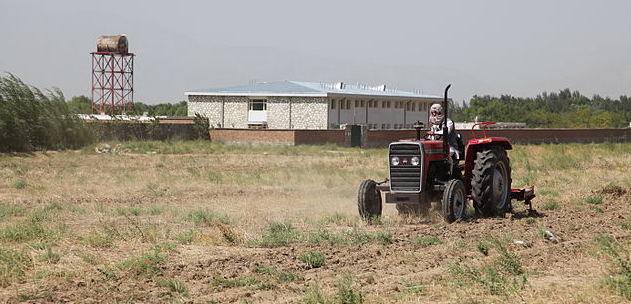
\includegraphics[width=\textwidth,trim=0 40 0 40, clip=true]{kapisa.png}
\caption{\textsl{University Farm}: al-Biruni University, Kapisa province, Afghanistan.
\label{farm}}
\end{figure}

\subsubsection*{Example 2} Although it may sound quaint, working farms could help to physically
sustain peeragogues, while putting the project's \patternname{Heartbeat} in tune with that of the seasons.  In the
current distributed mode, we tend our windowboxes and allotment gardens.   New developments
should unfold in a \emph{logical order growing out of the needs of the community} \cite[Chapter IX]{washington1986up}.
%% \begin{quote}
%% All of the industries at Tuskeege have been started in natural and
%% logical order growing out of the needs of a community settlement.  We
%% began with farming because we wanted something to
%% eat. \cite[Chapter IX]{washington1986up}
%% \end{quote}

\begin{framed}
\noindent 
\emph{What's Next in the Peeragogy Project}
\definecollection{HeartbeatWN}
\begin{collectinmacro}{\HeartbeatWN}{}{}
Identifying and fostering new \patternnameplural{Heartbeat} and new working groups can help make the community more robust.  This is the time dimension of spin-off projects described in \patternname{Reduce, reuse, recycle}.
\end{collectinmacro}
\HeartbeatWN
\end{framed}

%\newpage
